\section{Results}
\subsection{CFD Dataset}
\begin{figure}[htpb]
	\centering
	\includegraphics{Graphs/theta_peak_impulse_0.pdf}
	\caption{Contour plot peak impulse distribution overview of PE4 dataset}
	\label{fig:theta_peak_impulse_0}
\end{figure}
The CFD dataset obtained consists of 
\subsection{Randers-Pehrson Bannister (RPB) Model}
The specific impulse acting on a target is dependent on the angle of incidence of the shock front, theta, with respect to the normal of the target surface. 
From \textcite{randers-pehrsonAirblastLoadingModel1997},
\begin{equation}
	i = i_r cos^2\theta + i_{so}(1 + cos^2\theta - 2cos\theta). 
	\label{eq:RPB}
\end{equation}

Figure \ref{fig:RPB} shows the angle of incidence and slant distance for a point on a target subjected to a spherical air burst, a distance $R$ away from the target centre.
From trigonometry, we have that $\bar{R}^2 = R^2 + x^2 + y^2$, where $x \text{ and } y$ are horizontal and vertical distance from the centre of the target, and $cos \theta = R / \bar{R}$. 
 
\begin{figure}[htpb]
	\centering
	\includegraphics[scale=2, keepaspectratio]{Images/RPB.pdf}
	\caption{Angle of incidence and slant distance for a specific point on a square target}
	\label{fig:RPB}
\end{figure}

\subsection{Henrych Model}
From \textcite{henrychDynamicsExplosionIts1979}, we have a theoretical basis to calculate specific impulse distributions. 
The hypothesis of a constant velocity for out flowing particles is introduced:
\begin{equation}
	u = u_x = \text{ constant}.
\end{equation}
For a spherical charge, it is provided that
\begin{equation}
	i = \left(\frac{A_0W}{R^2}\right)cos^2\alpha,
	\label{eq:Henrych_sphere}
\end{equation}
where $R$ is the distance from charge centre to centre of target (shown also in Figure \ref{fig:RPB}) and given
\begin{equation}
	A_0 = \frac{N_{xW} + U_x}{4\pi}, 
\end{equation}
and $N_{xW}$ is the displacement velocity of the outburst surface.

\subsection{Model performance test}
Test the model with unseen data to demonstrate how this would work. 